\chapter{Opis implementacije}
\label{ch:implementacija}


This chapter describes how the four ray-traced effects and the shared denoiser are implemented inside
the Snowstorm engine, with the emphasis on the ray tracing itself and its cost rather than on every
engine subsystem.

\section{Snowstorm Engine (pregled)}
\label{sec:engine}

Snowstorm is a Vulkan engine the author wrote from scratch. This thesis uses it as the host for the
ray-tracing passes and does not treat the engine itself as the contribution. An EnTT-based
entity-component-system produces the per-frame render work. A backend-agnostic \texttt{Render/} layer
sits over a Vulkan RHI (volk, Vulkan Memory Allocator, spirv-reflect for descriptor layouts) in
\texttt{Platform/Vulkan/}, shaders are HLSL compiled to SPIR-V through dxc, and the ImGui editor hosts
the CVar console and the performance readouts (Section~\ref{sec:alati}).

The one part load-bearing for the RT path is the bindless descriptor model, which lets a single
hit-shading routine index any mesh's vertices, indices, and material without per-draw descriptor churn
(Section~\ref{sec:efekti}): each mesh exposes its vertex and index buffers by device address, and a
per-instance geometry table indexed by \texttt{instanceCustomIndex} lets the hit shader fetch the hit
triangle's attributes and its material at trace time. The Vulkan physical device is selected at startup
by index or name through a CVar, so the same binary runs on either GPU, which the cross-vendor
evaluation of Chapter~\ref{ch:analiza} depends on.

\section{Render graf i struktura frejma}
\label{sec:rendergraph}

The renderer is organized as a \texttt{RenderGraph}: passes are appended in order, each declaring the
textures it reads and writes, and the graph derives from those declarations both the Vulkan layout
barriers between them and a dependency DAG (\texttt{BuildDependencies}). Declaration order is a valid
topological order by construction, so the derived edges do not change what is correct, only what is
free to move: \texttt{BuildSchedule} pulls compute passes as early as their edges allow, gathering the
ray-traced chains into one contiguous run instead of leaving them split by the raster upsamples that
happen to sit between them. That contiguity is what makes async compute worthwhile, since otherwise
each chain would pay its own fork and join.

Two ordering constraints are derived rather than declared, since no texture edge expresses them.
Graphics passes keep their relative order, because they submit draws through a shared instance buffer at
a running cursor, so only compute passes are free to move. And a pass that writes the swapchain is
terminal, because the editor samples the viewport through ImGui bindings the graph cannot see. The
limitation is that the DAG is only as complete as the declarations: a pass touching an
acceleration structure, a bindless table, or a buffer carries a real ordering requirement that no edge
records, since only textures are tracked. The \texttt{render.graph.dumpdeps} CVar reports which passes
look unconstrained, so that gap is visible rather than latent.

Each pass is wrapped in a named GPU timestamp scope (\texttt{BeginGpuScope}), and those names are the
rows of Table~\ref{tab:pass-cost} in Chapter~\ref{ch:analiza}, so the graph structure and the finest
available measurement granularity are one and the same. The per-effect costs in Table~\ref{tab:cena}
are deliberately coarser, whole-frame differences rather than scope readings, since the default shadow
path has no scope of its own.

Table~\ref{tab:framegraph} gives the declared per-viewport order. Each ray-traced effect repeats the
same four-stage shape, trace, accumulate over time, filter spatially, and (for the half-resolution
ones) upsample, which is what lets one denoiser implementation serve all of them
(Section~\ref{sec:denoising}).

\begin{table}[tbp]
\caption[Prolazi po frejmu, redom]{Prolazi po frejmu redom kojim se izvr\v{s}avaju. Tri efekta se
rekonstrui\v{s}u pre osvetljavanja i ulaze u \texttt{Forward} kao teksture, a senke su izuzetak i
trasiraju se inline unutar \texttt{Forward} prolaza.}
\label{tab:framegraph}
\centering
\small
\begin{tabular}{@{}>{\raggedright\arraybackslash}p{2.9cm}@{\hspace{4mm}}>{\raggedright\arraybackslash}p{9.4cm}@{}}
\toprule
\textbf{Faza} & \textbf{Prolazi, redom} \\
\midrule
G-buffer & \texttt{DepthNormal} (dubina + geometrijska normala), \texttt{Velocity} (vektori kretanja) \\
\addlinespace[2pt]
GI (1/2 rez.) & \texttt{GI} $\rightarrow$ \texttt{GITemporal} $\rightarrow$ \texttt{GIDenoise} $\rightarrow$ \texttt{GIUpsample} \\
\addlinespace[2pt]
AO (1/2 rez.) & \texttt{AO} $\rightarrow$ \texttt{AOTemporal} $\rightarrow$ \texttt{AODenoise} $\rightarrow$ \texttt{AOUpsample} \\
\addlinespace[2pt]
Refleksije (puna) & \texttt{Reflection} $\rightarrow$ \texttt{ReflectionTemporal} (a-trous za refleksije je podrazumevano isklju\v{c}en) \\
\addlinespace[2pt]
Osvetljavanje & \texttt{Forward} (\texttt{DefaultLit}): early-Z prepass, nebo, inline zraci senke, i kombinovanje sa GI/AO/refleksijama \\
\addlinespace[2pt]
Post & \texttt{Upscale} $\rightarrow$ \texttt{TemporalResolve} (TAA) $\rightarrow$ tonemap $\rightarrow$ FXAA $\rightarrow$ \texttt{Sharpen} \\
\addlinespace[2pt]
Merenje & \texttt{Compare}, \texttt{Metrics} (PSNR, SSIM) \\
\bottomrule
\end{tabular}
\end{table}


Three of the four effects run as compute passes \emph{before} the forward pass, each writing a
denoised texture that the forward shader then samples. They need the depth+normal G-buffer as their
starting surface, so they follow \texttt{DepthNormal} but precede shading. Running them ahead of
forward lets it do a single lit combine (direct lighting plus the sampled indirect, AO, and
reflection) instead of interleaving trace and shade. This split of screen-space compute effects
feeding a forward combine follows how hybrid renderers such as Unreal's Lumen separate their screen
passes from hit lighting.

Shadows are the deliberate exception: the shadow ray is traced \emph{inline} inside the forward
shader, once per light per pixel, at full resolution and with no denoiser in between
(Section~\ref{sec:senke}). A visibility test is a single bit that is cheap to compute exactly and
expensive to reconstruct approximately, so for a handful of lights answering it in place beats
writing a buffer, filtering it, and reading it back. The cost is linear growth in light count, which
the alternative stochastic path of Section~\ref{sec:senke} exists to address.

GI and AO are traced at half resolution (\texttt{render.gi.scale}, \texttt{render.ao.scale}, both
0.5 by default) and bilaterally upsampled before the forward pass samples them, while reflections are
traced at full resolution. Half-res tracing is the single biggest cost lever for the two hemispheric
gather effects since it quarters the ray count, and Section~\ref{sec:cena} quantifies what it buys.
Which effects tolerate it is not arbitrary: reconstructing three pixels in four from their neighbours
is only safe when the signal varies slowly across the surface. Ambient occlusion and diffuse global
illumination are broad hemispherical averages, so adjacent pixels on the same wall genuinely receive
almost the same answer and interpolating introduces less error than the noise already present. A
shadow boundary is a step function and a reflection is view-dependent, so there a neighbouring pixel
can legitimately see something completely different, and halving the resolution destroys the detail
that made the effect worth tracing rather than blurring noise.

\section{Izgradnja struktura ubrzanja (BLAS/TLAS)}
\label{sec:accel}

Ray queries trace against the two-level structure described in Section~\ref{sec:accel-pregled}. Each
unique mesh owns one BLAS, built lazily on first use and cached on the mesh
(\texttt{Mesh::GetOrBuildBLAS}) with the \texttt{PREFER_FAST_TRACE} flag over opaque triangle
geometry referenced by device address (positions R32G32B32, 32-bit indices). Opaque meshes are
flagged \texttt{OPAQUE} so traversal skips the any-hit stage, while alpha-cutout (glTF MASK) materials
fall back to a minimal any-hit alpha test unless an opacity micromap is available. The TLAS holds one
instance per (Transform, Mesh) entity, each carrying its $3\times4$ world transform, a visibility
mask, its BLAS address, and an \texttt{instanceCustomIndex} set to the instance index so the hit
shader can resolve the geometry from a table (Section~\ref{sec:efekti}).

In \texttt{Sponza.world} the two-level structure buys nothing, since the model is authored as a
single unrepeated mesh set: 25 instances over 25 BLAS, one to one.
\texttt{Sponza-Motion.world} adds the four rotating props of Section~\ref{sec:motion}, four
transforms of one mesh, so its 29 instances share 26 BLAS. The instance count reported by
\texttt{TlasBuildSystem} climbs across rebuilds (6, 12, 18, 24, 25) as the meshes stream in, since a
mesh entity joins the structure only once its geometry is resident.

The TLAS is rebuilt in full on every frame the scene is marked dirty (\texttt{TlasBuildSystem}, in
the \texttt{PreRender} phase). There is no refit path: a dirty frame destroys and rebuilds the
structure (\texttt{MODE_BUILD_KHR}) behind a device wait. The dirty check excludes the camera, so a
scene whose geometry and transforms are static does not rebuild the TLAS even as the camera moves,
which is the common case for the benchmark scene. A full rebuild on every dynamic frame is heavier
than a refit would be. This is called out as a limitation in Chapter~\ref{ch:zakljucak} and was
chosen for implementation simplicity given that the test scenes are largely static.

\paragraph{Opacity micromaps za cutout geometriju.} On a device exposing
\texttt{VK\_EXT\_opacity\_micromap} (\texttt{render.omm}, on by default when supported), a cutout
material instead builds a second, non-opaque BLAS carrying an opacity micromap: a compute pass
(\texttt{OmmBake.comp}) bakes the material's albedo alpha into a per-microtriangle
opaque/transparent/unknown classification at a fixed subdivision level, using the same bird-curve
microtriangle indexing Khronos' reference implementation uses. Traversal then resolves opaque and
transparent microtriangles in hardware, so the any-hit alpha test runs only on the unknown (edge)
ones, whereas without the extension every cutout microtriangle pays it. The bake runs once per mesh and is
cached alongside the plain BLAS. Because it samples the resident albedo texture, it is deferred until
that texture has finished streaming in (an async load's placeholder is opaque, and baking against it
would cache a solid cutout permanently), with the any-hit fallback used meanwhile. Support is
driver-dependent as well as hardware-dependent: on the RDNA4 GPU used here the Vulkan driver does not
expose the extension despite the hardware, while the Blackwell NVIDIA GPU does, so the two vendors of
Chapter~\ref{ch:analiza} exercise different geometry paths for masked materials while producing the
same acceleration-structure query semantics.

The engine enables \texttt{VK_KHR_ray_query} and \texttt{VK_KHR_acceleration_structure} (plus
\texttt{VK_KHR_deferred_host_operations} for the build) but not the ray-tracing-pipeline extension.
There is no shader binding table: every trace is a \texttt{RayQuery} object created inside an
otherwise ordinary compute or fragment shader.

Where DXR would dispatch a hit group per geometry, here nothing is dispatched: the shader is handed
three integers and has to find the surface itself, walking the instance index through a
device-address \texttt{GeoRecord} table to the mesh's index and vertex buffers and its bindless
material (Figure~\ref{fig:hitresolve}). One routine, \texttt{ResolveHit} in
\texttt{RTHitShading.hlsli}, therefore resolves \emph{any} mesh in the scene with no per-geometry
shader and no descriptor rebinding, which is what makes a single \texttt{ShadeSurfaceHit} usable from
all four effects.

\begin{figure}[tbp]
\centering
\begin{tikzpicture}[>={Stealth[]}, font=\small, node distance=4mm,
  box/.style={draw, rounded corners, align=left, inner sep=4pt, text width=4.4cm},
  src/.style={box, fill=black!7}]
  \node[src] (hit) {\textbf{Poga\dj eni trougao}\\\footnotesize \texttt{instanceId}, \texttt{prim},
    \texttt{bary}};
  \node[box, below=8mm of hit] (rec) {\textbf{\texttt{GeoRecord}}\\\footnotesize adrese vertex i index
    bafera, indeks teksture, materijal};
  \node[box, right=16mm of rec] (idx) {\textbf{Index bafer}\\\footnotesize tri indeksa na
    \texttt{IndexAddress + prim*12}};
  \node[box, below=8mm of rec] (vtx) {\textbf{Vertex bafer}\\\footnotesize atributi, interpolirani
    baricentrima};
  \node[box, right=16mm of vtx] (tex) {\textbf{Bindless niz tekstura}\\\footnotesize
    \texttt{NonUniformResourceIndex}};
  \node[src, below=8mm of vtx] (out) {\textbf{\texttt{HitSurface}}\\\footnotesize albedo, normala,
    metalnost, hrapavost};
  \draw[->] (hit) -- node[right, font=\scriptsize] {tabela po adresi} (rec);
  \draw[->] (rec) -- (idx);
  \draw[->] (rec) -- (vtx);
  \draw[->] (idx) -- (vtx);
  \draw[->] (rec.east) to[out=-30, in=30] (tex.north east);
  \draw[->] (tex) -- (out);
  \draw[->] (vtx) -- (out);
\end{tikzpicture}
\caption[Razre\v{s}avanje pogotka kroz bindless tabelu geometrije]{Od poga\dj enog trougla do
osen\v{c}ene povr\v{s}i, bez shader binding table-a. \texttt{RayQuery} vra\'ca samo tri broja, a
\texttt{ResolveHit} od njih stiže do geometrije i materijala kroz tabelu indeksiranu sa
\texttt{instanceCustomIndex}. Indeks teksture nije uniforman unutar talasa, pa mora kroz
\texttt{NonUniformResourceIndex}.}
\label{fig:hitresolve}
\end{figure}

\section{\v{C}etiri efekta preko inline ray query}
\label{sec:efekti}

All four effects share the same core operation: construct a ray, create a \texttt{RayQuery} against
the scene TLAS, run its traversal loop, and act on the result. They differ on the four axes of
Table~\ref{tab:effect-params}, two of which are coupled: an effect that needs only a visibility answer
can stop at the first hit, which is both the cheaper traversal and the reason it can afford a lower
ray count than an effect that must shade what it finds.

\begin{table}[tbp]
\caption[Parametri \v{c}etiri efekta]{Kako se \v{c}etiri efekta razlikuju pri istoj inline ray query
operaciji. Broj zrakova i razmera su podrazumevane vrednosti odgovaraju\'cih CVar-ova. ,,Prvi
pogodak`` je \texttt{RAY\_FLAG\_ACCEPT\_FIRST\_HIT\_AND\_END\_SEARCH}, koji prekida obilazak \v{c}im
na\dj e bilo koji presek.}
\label{tab:effect-params}
\centering
\begin{tabular}{lllll}
\toprule
Efekat & zraka/piksel & obilazak & rezultat pogotka & razmera \\
\midrule
senke        & 4 po svetlu & prvi pogodak & vidljivost (0/1)        & 1.0 \\
AO           & 2           & prvi pogodak & okluzija + rastojanje   & 0.5 \\
refleksije   & 1           & najbli\v{z}i & osen\v{c}ena radijansa  & 1.0 \\
GI           & 2           & najbli\v{z}i & osen\v{c}ena radijansa  & 0.5 \\
\bottomrule
\end{tabular}
\end{table}

The effects that shade their hits (reflections and GI) share one routine, \texttt{ShadeSurfaceHit} in
\texttt{RTHitShading.hlsli}, which resolves the hit triangle through the bindless geometry table and
evaluates a single bounce, while shadows and AO need only a visibility answer and use the cheaper
any-hit traversal. Primary shading in the forward pass is a standard metallic-roughness Cook-Torrance model
(GGX distribution, Smith geometry with the Schlick-GGX approximation, Schlick Fresnel, Lambertian
diffuse), with the ambient term from a prefiltered environment cube and a precomputed BRDF lookup
table.

Secondary hits are shaded more cheaply, deliberately: \texttt{ShadeSurfaceHit} evaluates a Lambertian
diffuse term scaled by $(1 - \text{metallic})$, plus the surface's emissive term and an image-based
ambient fill, with no specular lobe at all, so a conductor seen in a reflection or through a GI bounce
returns black rather than a mirrored highlight. A second-bounce specular highlight is rare and
low-contrast once convolved by the denoiser, while a full BRDF evaluation at every hit would roughly
double the cost of the hit-shading path. The cost of the approximation is that metal-on-metal
interreflection is absent, which the path-traced reference in Section~\ref{sec:pathtracer} does
reproduce and which therefore shows up as a small systematic difference in the reflection metrics.

For the evaluation in Chapter~\ref{ch:analiza}, ambient occlusion, reflections, and global
illumination can each also be produced by a screen-space approximation, selected through a mode
setting (\texttt{render.ao.mode}, \texttt{render.reflections.mode}, \texttt{render.gi.mode}). SSAO,
SSR and SSGI read the same depth+normal G-buffer and write into the same slot their ray-traced
counterpart does (SSGI marches the depth buffer into the same half-res GI target, then flows through
the same temporal/denoise/upsample/forward tail), so the two versions of a given effect differ only
in how the signal is produced. They are the baselines of Section~\ref{sec:poredjenje}. SSGI's gather
has no device-support check and runs on any GPU, while ray-traced GI (mode 2) is the one that
degrades to off without ray-tracing support.

\subsection{Senke (RT shadows)}
\label{sec:senke}

Shadows are traced inline in the forward pass, once per light per pixel, at full resolution and
without an intervening denoiser (\texttt{DefaultLit.frag.hlsl} and the shared RT includes, in the
\texttt{SS_RAYTRACING} permutation). A shadow ray is a pure visibility test, so it uses the cheapest
traversal, \texttt{ACCEPT_FIRST_HIT_AND_END_SEARCH}. That traversal is not fully fixed-function,
since cutout geometry must be resolved in the shader: candidate hits on non-opaque triangles come back
through \texttt{q.Proceed()}, where the material's alpha is tested and the hit committed only if it
passes, and the first surviving hit marks the surface shadowed. The ray origin is offset along the
geometric normal and toward the light (\texttt{positionWS + Ng*0.02 + L*0.01}) to avoid
self-intersection (Listing~\ref{lst:shadow}).

The alternative the engine keeps is the raster shadow map, also the default and the fallback on a
device without ray tracing (Figure~\ref{fig:shadow-vs-map}). Intersecting the real geometry needs no
depth-bias tuning at all, although its price grows with light count where the map amortises over the
whole frame. Section~\ref{sec:analiza-shadow-strategy} measures that tradeoff.

\begin{figure}[tbp]
\centering
\begin{minipage}{0.48\textwidth}\centering
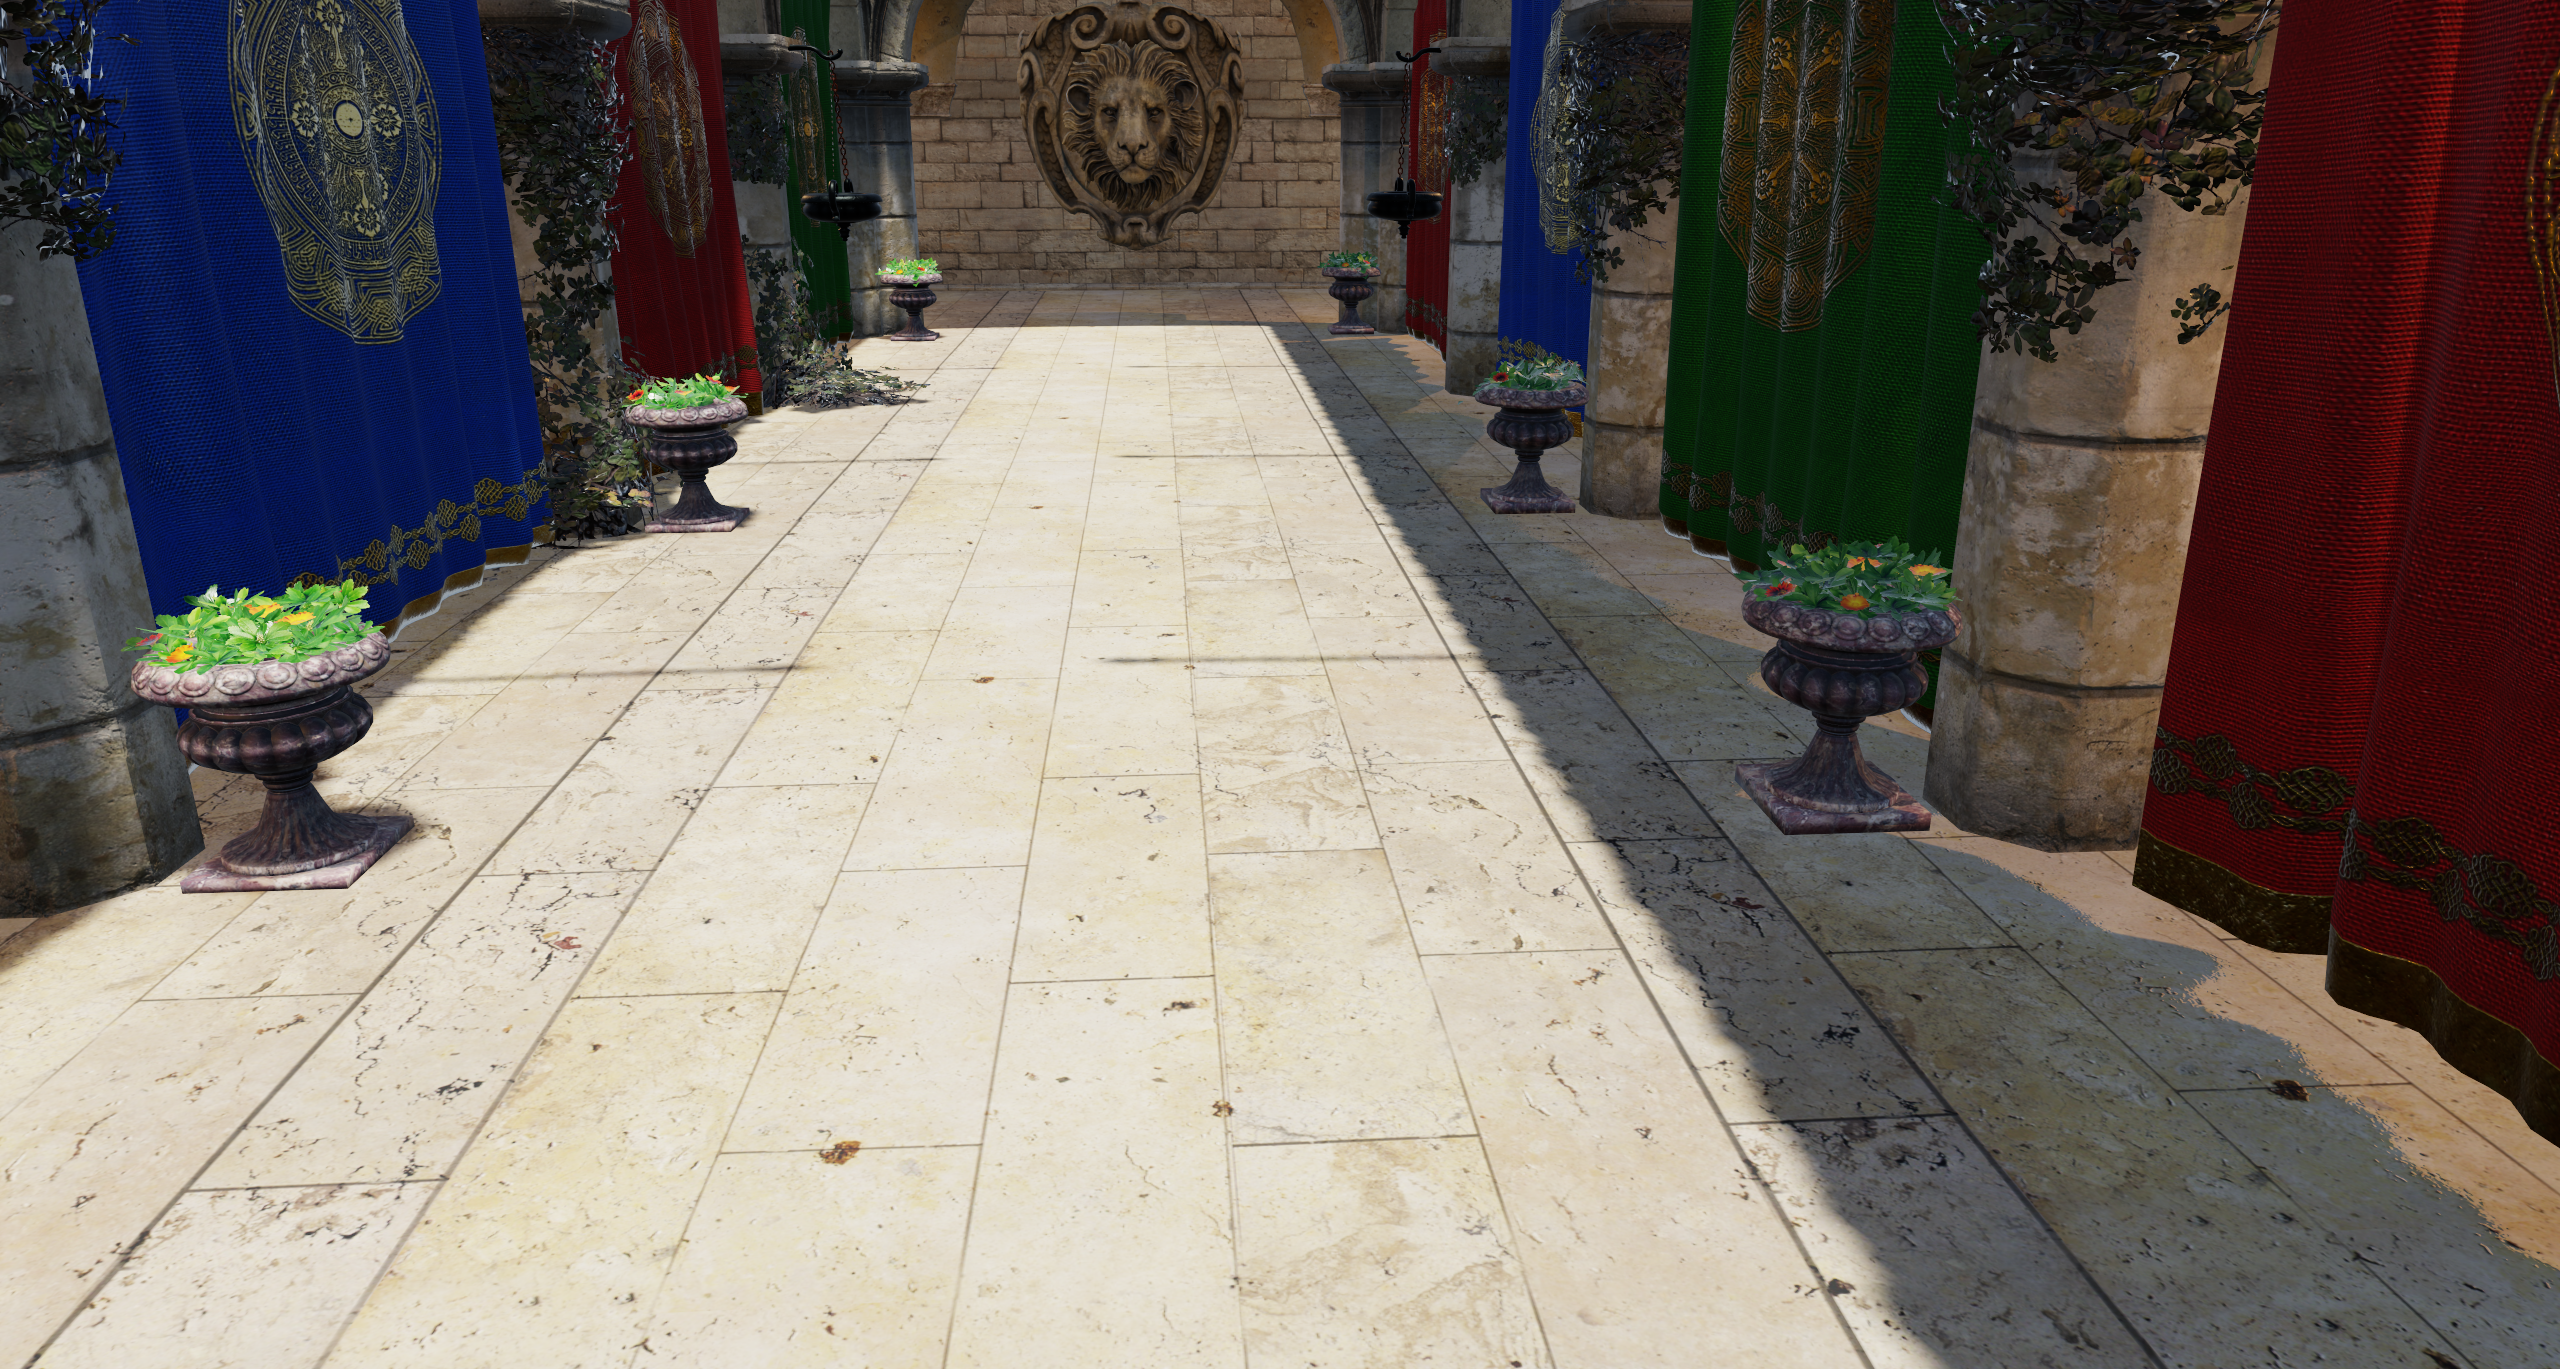
\includegraphics[width=\linewidth]{figures/shadow_map.png}\\{\small mapa senki (raster)}
\end{minipage}\hfill
\begin{minipage}{0.48\textwidth}\centering
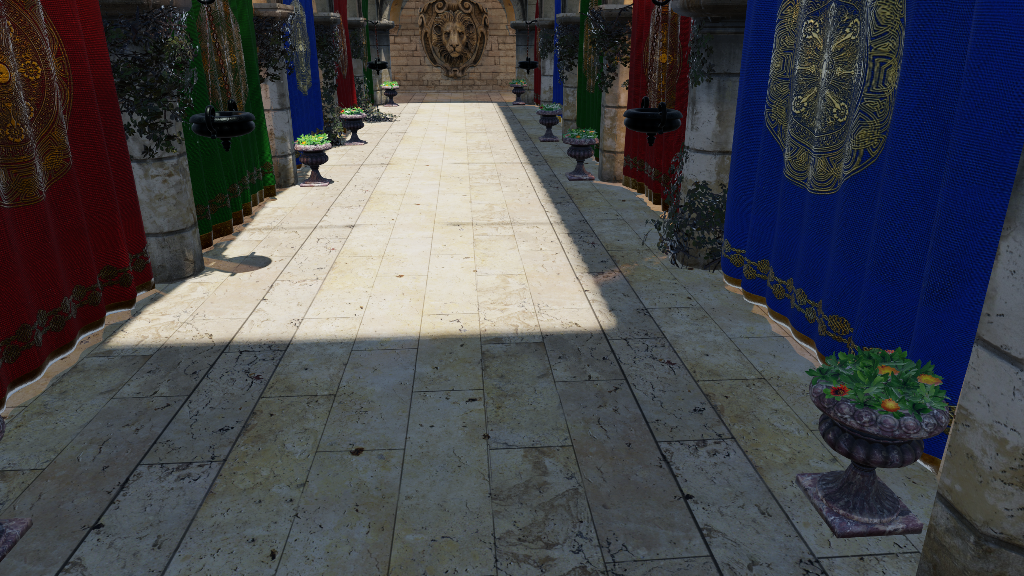
\includegraphics[width=\linewidth]{figures/shadow_rt.png}\\{\small trasirane senke}
\end{minipage}
\caption[Mapa senki naspram trasiranih senki]{Ista poza i isto svetlo, \texttt{render.shadows.mode}
1 naspram 2. Rasterska mapa ima kona\v{c}nu rezoluciju i pomeraj dubine, pa se kontaktne senke
razlivaju i ivice su mek\v{s}e nego \v{s}to geometrija nala\v{z}e, a trasirana verzija ih razre\v{s}ava
preko stvarne geometrije. Snimci su deterministi\v{c}ki (dva uzastopna snimka iste konfiguracije su
identi\v{c}na do bita), pa je svaka razlika izme\dj u panela stvarna.}
\label{fig:shadow-vs-map}
\end{figure}


\needspace{22\baselineskip}
\begin{lstlisting}[caption={Inline ray-query test vidljivosti za senku (HLSL).}, label={lst:shadow}]
RayQuery<RAY_FLAG_ACCEPT_FIRST_HIT_AND_END_SEARCH> q;
RayDesc ray;
ray.Origin    = positionWS + Ng * 0.02 + L * 0.01;
ray.Direction = L;
ray.TMin      = 0.0;
ray.TMax      = distanceToLight - 0.05;   // sun: effectively infinite
q.TraceRayInline(SceneTLAS, RAY_FLAG_NONE, 0xFF, ray);
while (q.Proceed())                       // alpha-test cutout candidates
{
    if (q.CandidateType() == CANDIDATE_NON_OPAQUE_TRIANGLE &&
        RTCommitCandidate(tableAddr, q.CandidateInstanceID(),
                          q.CandidatePrimitiveIndex(),
                          q.CandidateTriangleBarycentrics(), LinearSampler))
    {
        q.CommitNonOpaqueTriangleHit();
    }
}
bool shadowed = (q.CommittedStatus() == COMMITTED_TRIANGLE_HIT);
\end{lstlisting}

Two quality levels are exposed through the \texttt{render.shadow.soft} CVar. The hard path casts one
ray straight at the light, while the soft path casts \texttt{SHADOW_RAY_COUNT = 2} rays sampling, uniformly
by solid angle, the cone the source subtends at the shaded point (Figure~\ref{fig:shadow}), averaging
the hits into a penumbra factor in $[0,1]$. The cone is parameterised by the cosine of its half-angle:
$\cos(\tfrac{1}{2}\,\texttt{render.shadow.sun\_angle\_deg})$ for the sun, and
$\sqrt{1 - (r/d)^2}$ for a local light of radius \texttt{render.shadow.source\_radius} at distance
$d$, so a physically larger or nearer source gives a softer edge. Sampling the solid angle rather
than a tangent-plane disk is what makes the real-time penumbra agree with the path tracer's
next-event estimation at any cone width, instead of only in the small-angle limit where the two
parameterisations coincide. \texttt{SHADOW_RAY_COUNT} is a compile-time constant, a cost class rather
than a live knob. \texttt{render.shadows.rays} applies to the stochastic path below, not to this one.
Directions are decorrelated per pixel and per frame with an interleaved-gradient-noise hash, spreading
the two-sample penumbra across frames for the temporal accumulator to resolve
(Sections~\ref{sec:denoising} and \ref{sec:taa}).

\begin{figure}[tbp]
\centering
\begin{tikzpicture}[>={Stealth[]}]
  \draw[thick] (-2.6,0) -- (2.6,0);                      % surface
  % light-source disk (perpendicular to L), drawn as a circle
  \draw[fill=black!8] (2.7,2.4) circle (0.45);
  \node[font=\scriptsize, align=center] at (2.7,3.25) {izvor\\(polupre\v{c}nik $r$)};
  % direction to the light centre
  \draw[dashed] (0,0) -- (2.7,2.4);
  \node[font=\scriptsize] at (1.55,1.05) {$L$};
  % sample rays fanning to distinct points across the disk
  \draw[->, black!65] (0,0) -- (2.72,2.83);
  \draw[->, black!65] (0,0) -- (3.08,2.22);
  \draw[->, black!65] (0,0) -- (2.36,2.06);
  \draw[<->, black!45] (2.62,2.72) arc (46:38:3.6);
  \node[font=\scriptsize, black!55] at (3.02,2.52) {$\theta/2$};
  \fill (0,0) circle (1.7pt) node[below=3pt] {$P$};
\end{tikzpicture}
\caption{Meke senke: iz ta\v{c}ke $P$ se zraci uzorkuju ravnomerno po prostornom uglu unutar konusa
koji izvor zaklapa oko pravca $L$, sa polovinom ugla $\theta/2$ odre\dj enom polupre\v{c}nikom
izvora $r$ i rastojanjem. Udeo neblokiranih zraka daje penumbru.}
\label{fig:shadow}
\end{figure}

Penumbra width is $2H\tan(\theta/2)$ in the occluder-to-receiver distance $H$ and the source's
angular size $\theta$, so Figure~\ref{fig:shadow-hs} frames the sunlit floor strip: the sun is the
only light here with a distant occluder, its transverse edge cast by the roof light-well lip about
10.4 units above the floor, while the four enabled torches sit a couple of units from the walls they
light. At the sun's true angular diameter that penumbra is roughly 36 pixels of a 2560-wide capture
and disappears once scaled into the page, so the figure raises
\texttt{render.shadow.sun\_angle\_deg} to $3^\circ$ and says so in its caption. Widening
\texttt{render.shadow.source\_radius} instead would be the wrong control, for a reason that is also a
limitation. Cone samples falling below the shading normal's horizon are skipped while the
average still divides by the full sample count, which is deliberate (counting them lit is the leak
that next-event estimation rejects in the path tracer), although it means a wider cone also darkens
grazing surfaces systematically. At a 1.5-unit radius that darkening accounts for about three quarters
of the frame difference and swamps the penumbra it was meant to show. The near-vertical sun meets the
floor at $\mathbf{n}\cdot\boldsymbol{\omega} \approx 1$ and avoids it, since no sample is
horizon-rejected there.

\begin{figure}[tbp]
\centering
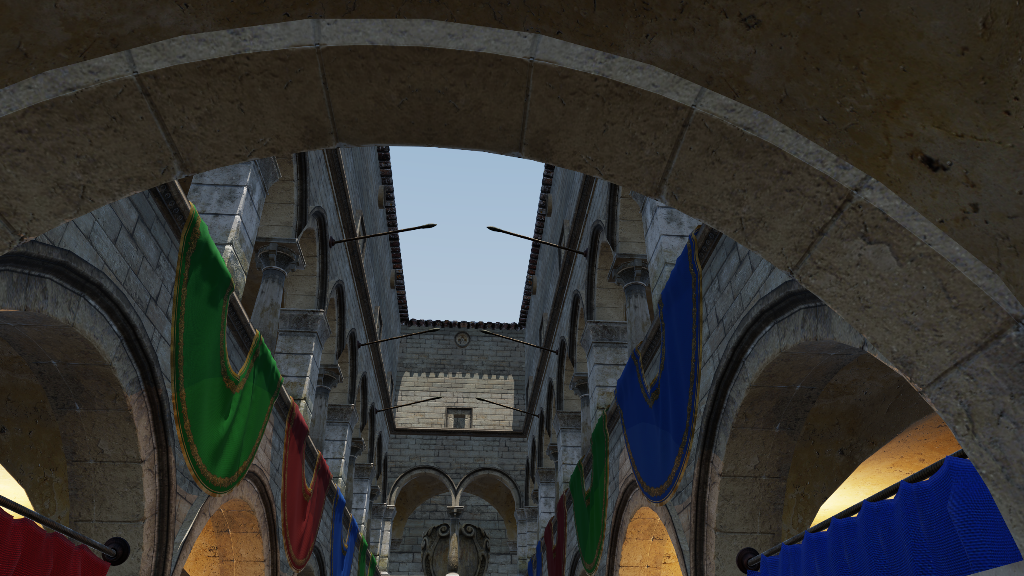
\includegraphics[width=0.48\textwidth]{figures/shadow_hard.png}\hfill%
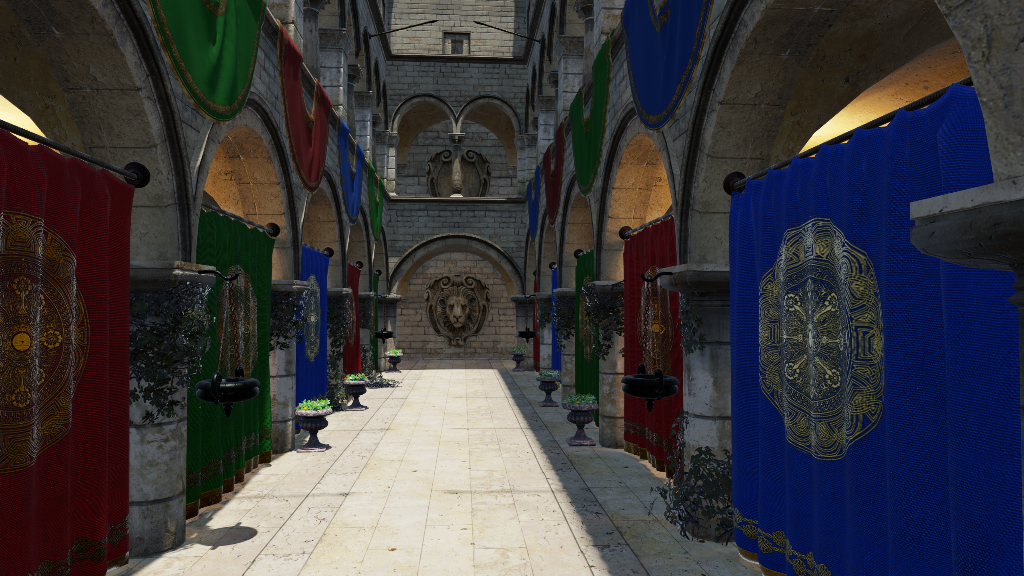
\includegraphics[width=0.48\textwidth]{figures/shadow_soft.png}
\caption{Tvrde (levo) naspram mekih (desno) ray-traced senki na osun\v{c}anoj traci poda: jedina
razlika je \texttt{render.shadow.soft}. Uglovni pre\v{c}nik sunca je podignut na $3^\circ$, oko
\v{s}est puta iznad fizi\v{c}kih $0{,}53^\circ$, jer je na stvarnoj vrednosti penumbra u\v{z}a od
onoga \v{s}to se vidi u \v{s}tampi.}
\label{fig:shadow-hs}
\end{figure}

\paragraph{Stohasti\v{c}ka alternativa.} Tracing one ray per light per pixel is exact but scales
linearly with light count, which does not survive a scene lit by hundreds of sources. The engine
therefore implements a second strategy, enabled by \texttt{render.shadows.stochastic} and off by
default, following the MegaLights approach: each pixel uses resampled importance sampling to pick
\emph{one} light with probability proportional to its unshadowed contribution, traces
\texttt{render.shadows.rays} rays at that light alone, and writes a single aggregate visibility ratio.
The estimate is unbiased but extremely noisy, since one pixel's sample says nothing about which light
its neighbour chose, so this path necessarily runs as its own half-resolution chain,
\texttt{RTShadow} $\rightarrow$ \texttt{ShadowTemporal} $\rightarrow$ \texttt{ShadowDenoise0..2}
$\rightarrow$ \texttt{ShadowUpsample}, reusing the shared denoiser, with a parallel
demodulated-specular chain for the specular occlusion term. Those passes carry their own GPU timestamp
scopes, which Section~\ref{sec:cena} accounts for separately from the forward pass. Its cost is
constant in light count, which is the whole point: the inline path wins for a handful of lights and
loses for many. Section~\ref{sec:analiza-shadow-strategy} measures the crossover on this scene, and
the debug views expose the aggregate visibility buffer before and after filtering
(Figure~\ref{fig:shadow-denoise-ab}), where one sample per pixel is nearly binary noise.

\begin{figure}[tbp]
\centering
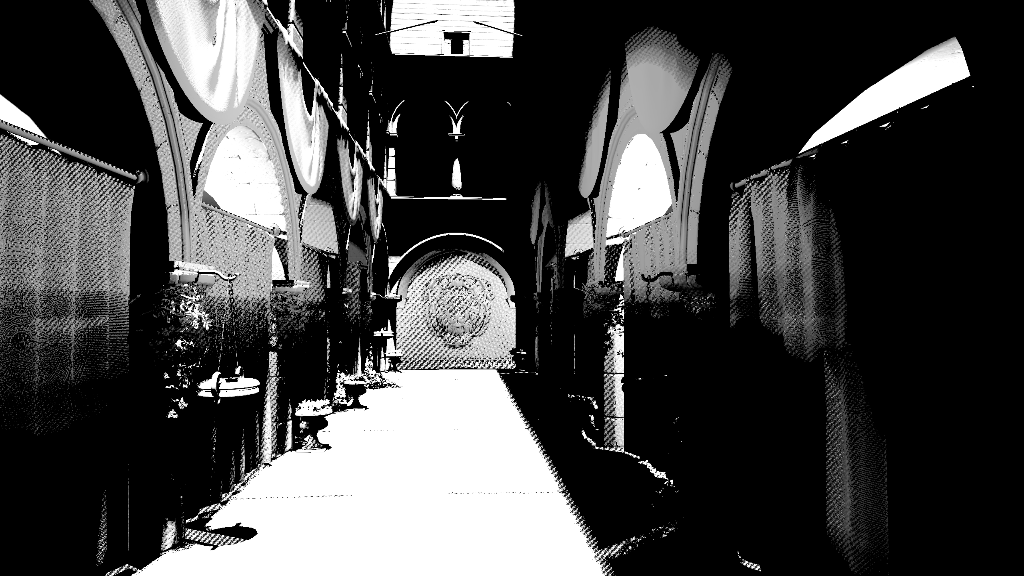
\includegraphics[width=0.48\textwidth]{figures/dbg_shadow_raw.png}\hfill%
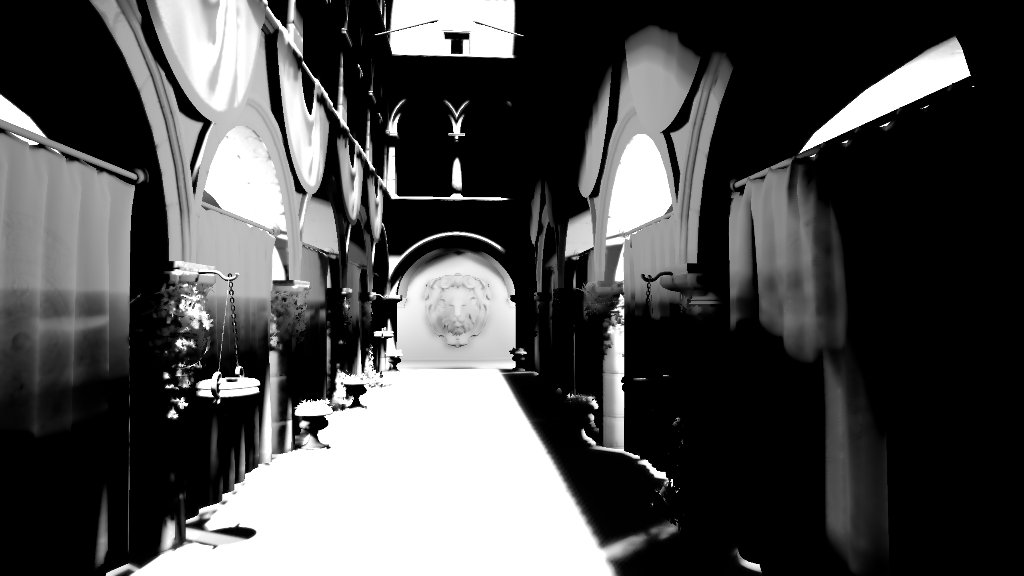
\includegraphics[width=0.48\textwidth]{figures/dbg_shadow_denoised.png}
\caption{Stohasti\v{c}ki agregatni odnos vidljivosti pre (levo) i posle (desno) temporalne
akumulacije i a-trous filtra (\texttt{render.debugview} 8 i 9). Belo je potpuno osvetljeno, crno
potpuno u senci. Levo se vidi da jedan uzorak po pikselu daje skoro binarni \v{s}um.}
\label{fig:shadow-denoise-ab}
\end{figure}

\subsection{Ambijentalna okluzija (AO)}

Ambient occlusion is a compute pass (\texttt{AO.comp.hlsl}) run at half resolution. Each pixel
reconstructs world position from the depth G-buffer and casts \texttt{render.ao.rays} short rays
(default 2, clamped to $[1,16]$) over the cosine-weighted hemisphere around the geometric normal,
rotated per pixel by interleaved gradient noise, using the same
\texttt{ACCEPT_FIRST_HIT_AND_END_SEARCH} visibility traversal as shadows. Rays are limited to
\texttt{render.ao.radius}, and a hit contributes \texttt{1 - saturate(t / AORadius)}, so nearer occluders
darken more, and the result is scaled by \texttt{render.ao.intensity} (Listing~\ref{lst:ao}).


\needspace{17\baselineskip}
\begin{lstlisting}[caption={AO uzorkovanje hemisfere (HLSL, karakteristi\v{c}an ise\v{c}ak).}, label={lst:ao}]
float occlusion = 0.0;
for (uint k = 0; k < RayCount; ++k)
{
    float3 dir = CosineHemisphere(k, RayCount, ign, N); // cosine-weighted, IGN-rotated around N
    RayQuery<RAY_FLAG_ACCEPT_FIRST_HIT_AND_END_SEARCH> q;
    RayDesc ray = MakeRay(positionWS + N * 0.02, dir, 0.0, AORadius);
    q.TraceRayInline(SceneTLAS, RAY_FLAG_NONE, 0xFF, ray);
    while (q.Proceed()) { /* alpha-test cutout candidates, as in Listing 3.1 */ }
    if (q.CommittedStatus() == COMMITTED_TRIANGLE_HIT)
        occlusion += 1.0 - saturate(q.CommittedRayT() / AORadius);
}
occlusion = 1.0 - occlusion / RayCount;
\end{lstlisting}

The pass writes \texttt{float4(ao, ao, ao, meanHitT)}, the alpha channel carrying the mean
distance to the occluders. That alpha feeds a hit-distance-guided edge-stopping term in the
denoiser (Section~\ref{sec:denoising}), the same idea NVIDIA's ReBLUR denoiser \cite{nvidia_nrd} uses
to scale the spatial filter by how far the occluder was. The term is implemented but disabled by
default on every signal, AO included: at two rays per pixel the hit distance is itself too noisy to
steer the filter, and a wrong steer is worse than none. The half-resolution result is denoised and
bilaterally upsampled before the forward pass multiplies it into the ambient term
(Figure~\ref{fig:ao}).

\begin{figure}[tbp]
\centering
\begin{tikzpicture}[>={Stealth[]}]
  \draw[thick] (-2.7,0) -- (2.7,0);
  \draw[dashed] (-1.9,0) arc (180:0:1.9);
  \draw[->, thick] (0,0) -- (0,2.25) node[above] {$N$};
  \foreach \a in {30,60,90,120,150} \draw[->, black!60] (0,0) -- (\a:1.9);
  \draw[fill=black!12] (0.85,0.55) rectangle (1.3,1.25);
  \draw[thin] (1.3,1.1) -- (2.05,1.6);
  \node[font=\scriptsize, anchor=west] at (2.05,1.6) {okluder};
  \fill (0,0) circle (1.7pt) node[below=3pt] {$P$};
\end{tikzpicture}
\caption{Uzorkovanje po hemisferi za AO: iz ta\v{c}ke $P$ se baca vi\v{s}e kratkih zraka po hemisferi
oko normale $N$. Udeo zraka koji u zadatom polupre\v{c}niku pogodi geometriju daje okluziju.}
\label{fig:ao}
\end{figure}

\subsection{Refleksije (reflections)}

Reflections are a compute pass (\texttt{Reflection.comp.hlsl}) run at full resolution, the only
ray-traced effect not traced at half res, since reflection detail is view-dependent and does not
tolerate the blur that half-res tracing plus upsampling introduces. Each pixel reconstructs world
position and reflects the view vector about the normal-mapped shading normal (read from a separate
shading-normal G-buffer, not the geometric normal, so normal maps are mirrored correctly). It needs
the closest hit, so unlike the visibility queries it uses a plain \texttt{RayQuery<RAY_FLAG_NONE>}
and runs traversal to completion.

Glossy reflections are approximated by jittering each ray inside a cone whose half-angle scales with
surface roughness (\texttt{roughness * ReflConeScale}), averaged over \texttt{render.reflections.rays}
(default 1), while a mirror surface (\texttt{roughness == 0}) collapses to one sharp ray. Hits are
shaded by \texttt{ShadeSurfaceHit} (sun lighting with its own shadow ray, the hit surface's emissive
term, image-based ambient), and a miss samples the prefiltered sky cube. Unlike the GI pass below, reflections
do not sample the scene's local point and spot lights at the hit: the same importance-sampled
local-light estimator was measured here too and showed no quality gain for twice the GI side's cost,
so it is compiled out of this pass entirely. The pass writes raw reflected radiance plus hit distance,
while the Fresnel term, the BRDF weighting, and \texttt{render.reflections.intensity} are applied
afterward in the forward pass (Figure~\ref{fig:refl}).

\begin{figure}[tbp]
\centering
\begin{tikzpicture}[>={Stealth[]}]
  \draw[thick] (-2.7,0) -- (2.7,0);
  \draw[->, thick] (0,0) -- (0,2.2) node[above] {$N$};
  \draw[->, black!55] (-2.05,2.05) -- (0,0); \node[font=\scriptsize] at (-1.55,1.35) {$V$};
  \foreach \a in {50,62,74} \draw[->, black!65] (0,0) -- (\a:2.15);
  \draw[dashed] (0,0) -- (62:2.3) node[above right, font=\scriptsize] {$R$};
  \node[font=\scriptsize, align=center] at (2.0,1.05) {konus\\(hrapavost)};
  \fill (0,0) circle (1.7pt) node[below=3pt] {$P$};
\end{tikzpicture}
\caption{Refleksije: pravac odbijanja $R$ vektora pogleda $V$ oko normale $N$. Glatka povr\v{s}ina
daje jedan o\v{s}tar zrak, a hrapava uzorkuje konus oko $R$.}
\label{fig:refl}
\end{figure}

Figure~\ref{fig:refl-onoff} shows the contribution of the pass. The cone itself
(Figure~\ref{fig:refl-cone}) resists the obvious measurement: sweeping
\texttt{render.reflections.cone\_scale} from 0 (a pure mirror ray) to 3 changes the finished frame by
a mean of only 0.16 levels out of 255, across six camera poses tried. The cause is that the reflection
is a small additive term next to direct lighting, so the composited image hides it. Measured on the
reflection buffer before compositing, the same A/B moves 43.7 levels and drops the buffer's
high-frequency energy from \hfConeSharp{} to \hfConeGlossy{}, a factor of 275 more signal than the
composited comparison shows. The figure therefore uses the isolated buffer, for the same reason the
effect gallery in Section~\ref{sec:cena} does: a term that is small in the final image can still be
the whole content of its own intermediate.

\begin{figure}[tbp]
\centering
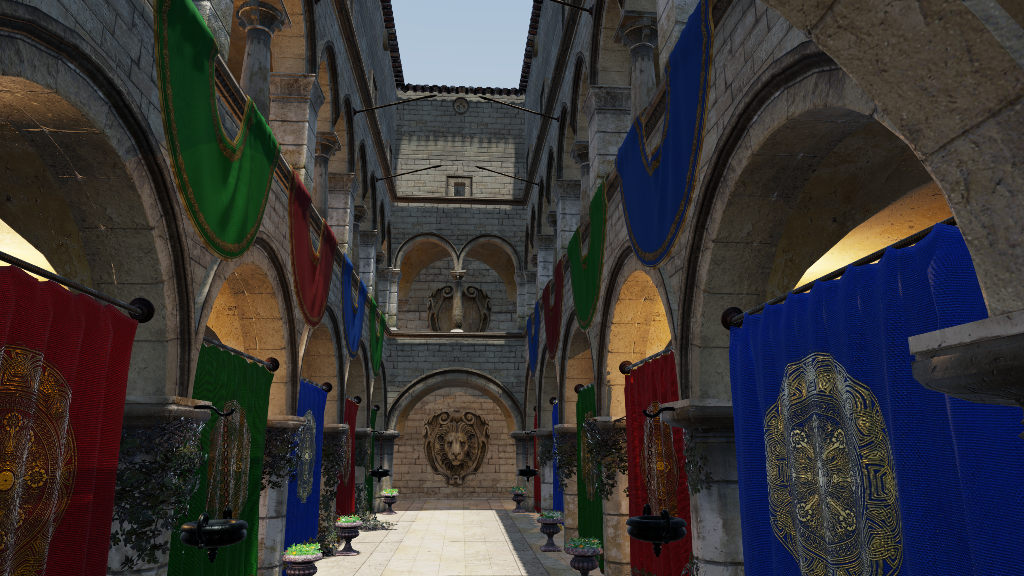
\includegraphics[width=0.48\textwidth]{figures/refl_off.png}\hfill%
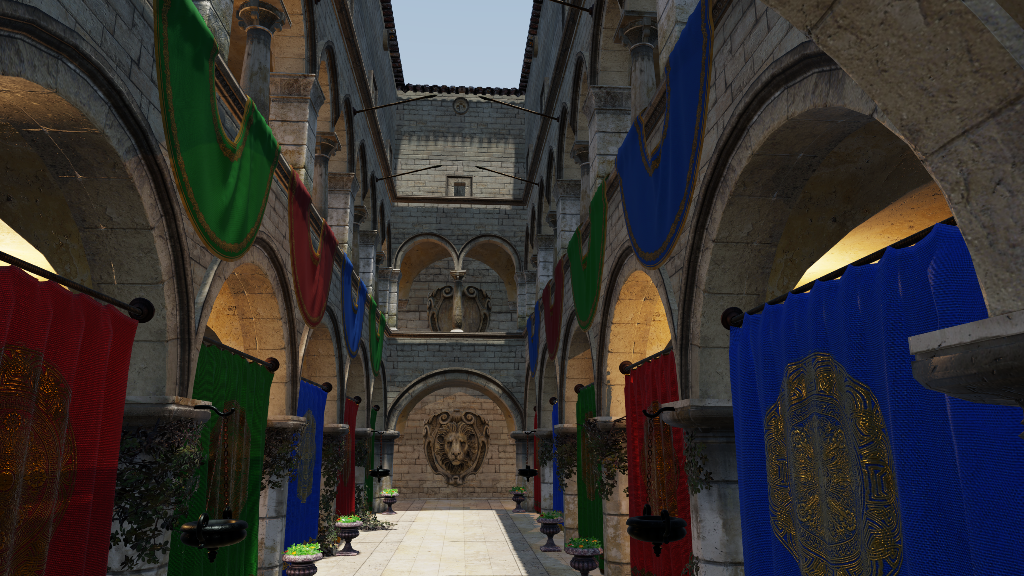
\includegraphics[width=0.48\textwidth]{figures/refl_rt.png}
\caption{Bez refleksija (levo) naspram ray-traced refleksija (desno), pri uglu gledanja blizu
tangentnog gde je Fresnel-ov doprinos najve\'ci. Sjaj na draperijama i kamenu je razlika koju
donosi prolaz.}
\label{fig:refl-onoff}
\end{figure}

\begin{figure}[tbp]
\centering
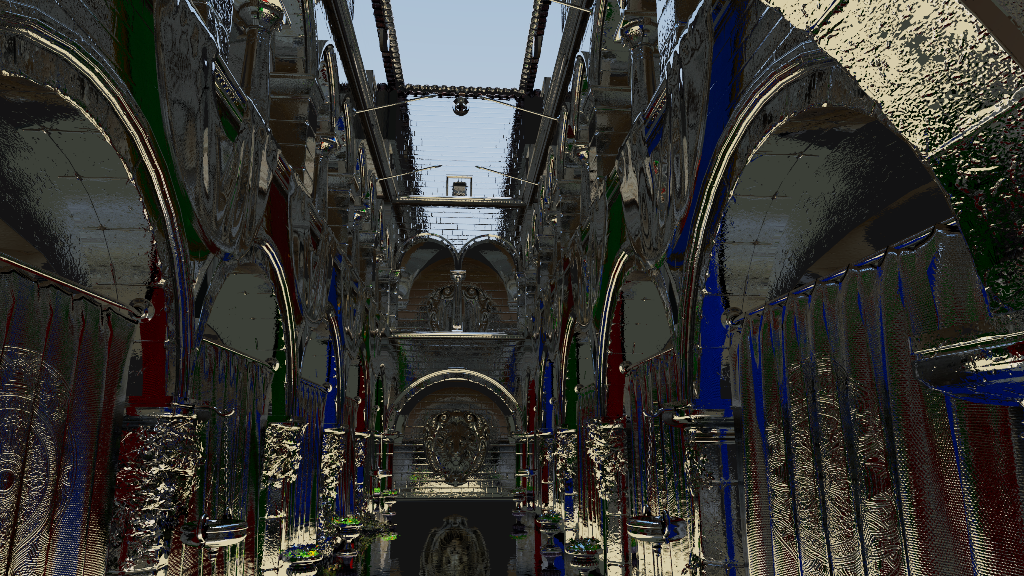
\includegraphics[width=0.48\textwidth]{figures/cone_sharp.png}\hfill%
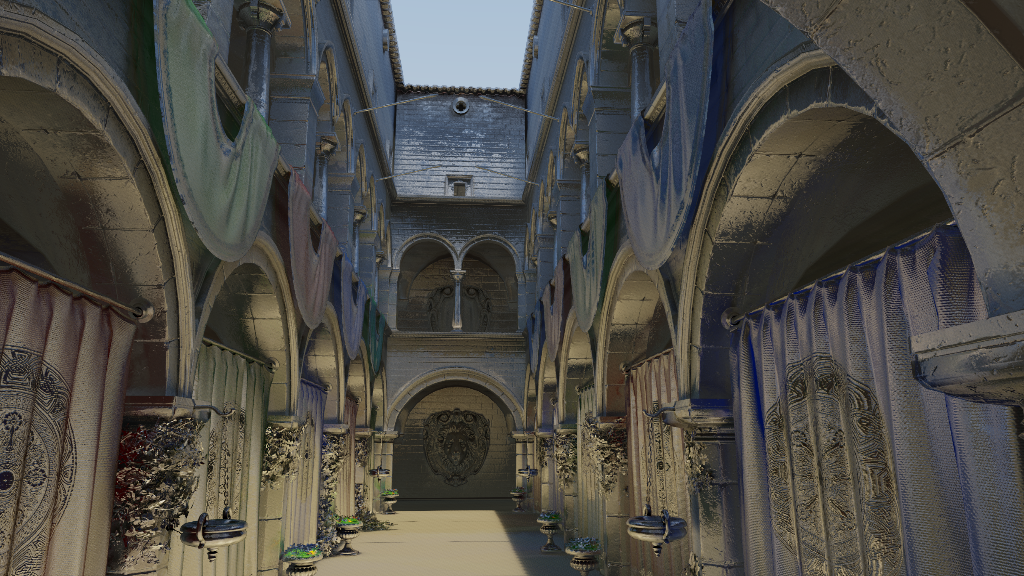
\includegraphics[width=0.48\textwidth]{figures/cone_glossy.png}
\caption{Reflektovana radijansa pre kombinovanja (\texttt{render.debugview} 3): o\v{s}tar ogledalski
zrak, \texttt{cone\_scale} 0 (levo), naspram konusa \v{s}irenog hrapavo\v{s}\'cu, \texttt{cone\_scale}
3 (desno). U gotovoj slici se ova razlika ne vidi jer je refleksija mali aditivni \v{c}lan pored
direktnog osvetljenja, a u sopstvenom baferu ona je ceo sadr\v{z}aj.}
\label{fig:refl-cone}
\end{figure}

\subsection{Globalno osvetljenje (GI)}

Global illumination is the most expensive effect: a compute pass (\texttt{GI.comp.hlsl}) run at half
resolution that computes one bounce of diffuse indirect light. It samples the hemisphere exactly as
AO does, \texttt{render.gi.rays} rays (default 2) out to \texttt{render.gi.range}. The difference is
what a ray returns. A miss samples the sky cube, and each hit is shaded by
\texttt{ShadeSurfaceHit}: the sun with its own shadow ray,
the hit surface's emissive term, an image-based ambient fill, and, when \texttt{render.rt.hit_lights}
is on (the default), one of the scene's point and spot lights. That light is importance-sampled in
proportion to its unshadowed contribution at the hit and confirmed with its own shadow ray, an
unbiased single-sample estimator (the same one \texttt{RTShadowPass} uses, in the spirit of UE5's
MegaLights) whose cost is constant in the light count, unlike a full next-event-estimation sum over
every light, which would multiply the ray budget at every secondary hit. This term is GI-only, and the
routine does not re-trace beyond these shadow rays, so the evaluation remains one bounce.

The pass outputs incoming irradiance only, without the receiver's albedo, which is multiplied in at
full resolution in the forward pass. This is the demodulated-irradiance convention that both the SVGF
denoiser and probe systems such as DDGI/RTXGI \cite{majercik2019ddgi, nvidia_rtxgi} rely on: filtering
irradiance rather than final color keeps the denoiser's edge-stopping from being misled by albedo
texture detail. The forward pass then replaces its flat ambient term with this ray-traced indirect,
the same substitution Lumen and RTXGI make \cite{epic_lumen}. At two rays per pixel and half
resolution (Figure~\ref{fig:gi}) the raw output is usable only after the temporal-plus-spatial denoise
of Section~\ref{sec:denoising}.

\begin{figure}[tbp]
\centering
\begin{tikzpicture}[>={Stealth[]}]
  \draw[thick] (-2.9,0) -- (2.9,0);
  \draw[dashed] (-2.1,0) arc (180:0:2.1);
  \draw[->, thick] (0,0) -- (0,2.45) node[above] {$N$};
  \foreach \a in {35,70,110,145} \draw[->, black!60] (0,0) -- (\a:2.1);
  \foreach \a in {35,70,110,145} \fill[black!30] (\a:2.1) circle (2.4pt);
  \fill (0,0) circle (1.7pt) node[below=3pt] {$P$};
\end{tikzpicture}
\caption{Globalno osvetljenje: kosinusno uzorkovanje hemisfere oko $N$ iz ta\v{c}ke $P$. Svaki zrak
koji pogodi geometriju vra\'ca radijansu (jedno odbijanje).}
\label{fig:gi}
\end{figure}

Figure~\ref{fig:gi-onoff} shows the scene without and with ray-traced global illumination.

\begin{figure}[tbp]
\centering
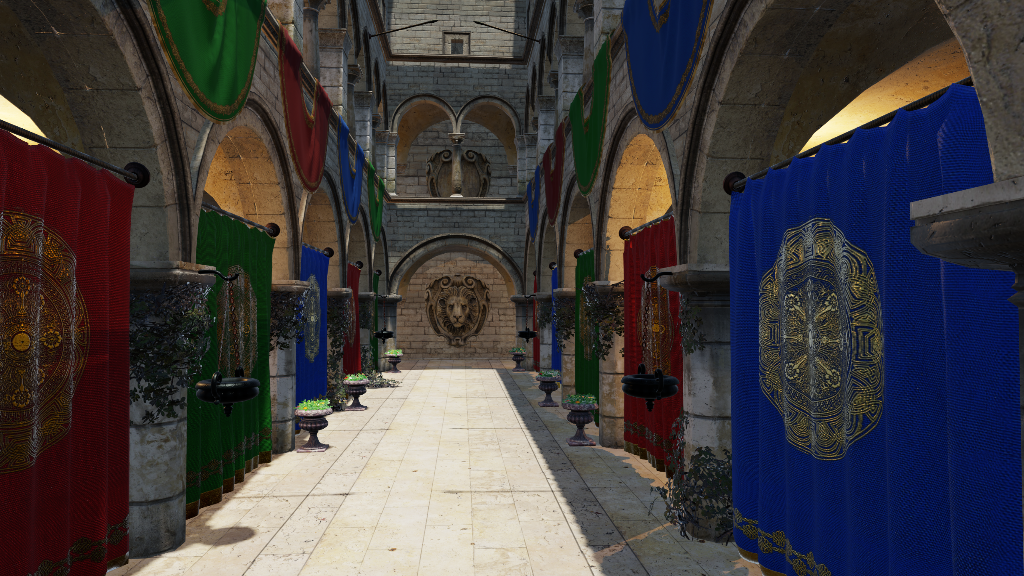
\includegraphics[width=0.82\textwidth]{figures/gi_off.png}

\vspace{6pt}

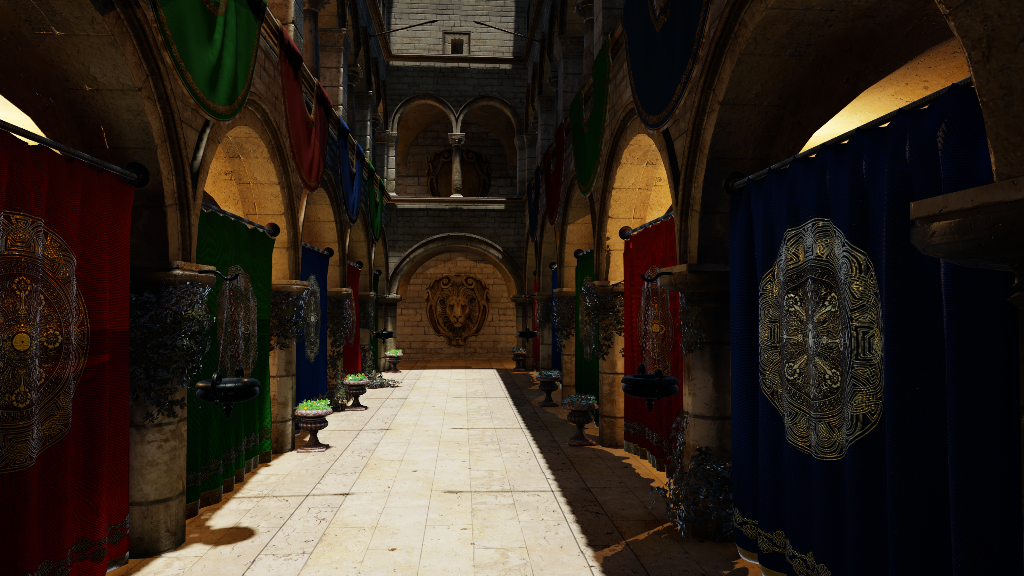
\includegraphics[width=0.82\textwidth]{figures/gi_on.png}
\caption{Scena bez (gore) i sa (dole) globalnim osvetljenjem: jedan difuzni indirektni odboj daje
prelivanje boja i popunu u senkama.}
\label{fig:gi-onoff}
\end{figure}

\section{Denoising (SVGF)}
\label{sec:denoising}

Each effect here estimates an integral over incoming directions from one or two samples, and
$\sqrt{n}$ convergence means samples alone cannot buy a clean image inside a frame budget. The
missing samples do exist, just not in this pixel and this frame: neighbouring pixels usually look at
nearly the same surface, and the previous frame usually contains the same surface one small camera
motion away. A denoiser borrows those samples spatially and temporally while refusing to borrow
across a real edge, where the neighbour is a different surface and averaging would smear the image.
Deciding what counts as "the same surface" is the entire difficulty, and it is why a denoiser needs
the G-buffer's depth and normals rather than just the colour.

Snowstorm implements a variant of Spatiotemporal Variance-Guided Filtering (SVGF)
\cite{schied2017svgf}, the standard real-time reconstruction filter for path-traced effects, as a
single signal-agnostic component. One \texttt{Denoiser} class (\texttt{Render/Denoiser.\{hpp,cpp\}})
drives a temporal accumulation and a spatial \`a-trous filter, with all per-viewport GPU state
(history, moments, scratch ping-pong textures) in a \texttt{DenoiserInstance} component the caller
owns. It is instantiated four times, for shadows, GI, AO, and reflections, each with its own
configuration but identical code (Figure~\ref{fig:svgf}). The reuse is possible because the noisy
estimate, its variance inputs, and the depth/normal G-buffer are the only signal-specific data. The
hit-distance
edge-stopping weight is wired up for every signal but left at zero by default, so that term is a
no-op in the measured configuration. The stochastic shadow path instead sizes its kernel by occluder
distance directly, in the NRD SIGMA style, through \texttt{render.shadows.denoise.penumbra}.
Reflections reuse GI's temporal shader, a limitation since a reflection history has view-dependent
content that a diffuse-tuned reprojection does not perfectly handle.

\begin{figure}[tbp]
\centering
\begin{tikzpicture}[>={Stealth[]}, node distance=5mm,
  box/.style={draw, rounded corners, align=center, text width=10.6cm, inner sep=4pt, font=\small}]
  \node[box] (in)  {Noisy input (GI and AO at half resolution, reflections at full)};
  \node[box, below=of in]  (tp) {\textbf{Temporal:} reproject by motion vectors, accumulate history
    (up to 32 frames), estimate per-pixel variance};
  \node[box, below=of tp]  (at) {\textbf{\`A-trous spatial filter:} 3 iterations by default (up to 5),
    stride $1, 2, 4, \dots$; edge-stopping on normal, depth, and variance};
  \node[box, below=of at]  (out){Denoised, then upsampled, into the Forward pass};
  \draw[->] (in) -- (tp); \draw[->] (tp) -- (at); \draw[->] (at) -- (out);
\end{tikzpicture}
\caption{SVGF denoiser: temporalna akumulacija sa procenom varijanse, zatim varijansom-vo\dj en
\`a-trous prostorni filter, deljen izme\dj u GI, AO i refleksija.}
\label{fig:svgf}
\end{figure}

\subsection{Temporalna akumulacija}

The temporal pass (\texttt{GITemporal.comp.hlsl}, at trace resolution) reprojects the previous
frame's result by the motion vectors (\texttt{prev_uv = uv - velocity}) and blends it with the
current noisy input. Off-screen samples and the first frame reset to the current input, and a
relative-depth test rejects disoccluded pixels. The blend follows SVGF's history-length scheme: a
per-pixel accumulated history length, capped at 32 frames, sets the blend weight
\texttt{max(alphaMin, 1 / historyLength)}, so a freshly disoccluded pixel weights the current frame
heavily while a long-lived pixel averages many frames. First and second luminance moments accumulate
with the same weight, and their difference is the temporal variance that guides the spatial filter.
Pixels too young for a stable temporal variance (history under four frames) fall back to a
$7\times7$ spatial variance estimate.

A neighborhood color clamp is added over stock SVGF: the reprojected history is clipped toward the
mean of a $3\times3$ current-frame neighborhood, weakened when the pixel is static and tightened when
it moves. This TAA-style clamp suppresses ghosting on moving edges and in reflections, where
depth/normal rejection alone is insufficient.

\subsection{Prostorni \`a-trous filter}

The spatial pass (\texttt{GIDenoise.comp.hlsl}) is the \`a-trous wavelet filter at the core of SVGF:
each iteration is a $5\times5$ tap gather with a B3-spline kernel, and successive iterations double
the tap stride (\texttt{step = 1 << i}). The engine runs up to five iterations, configurable per
signal. At the default three (Figure~\ref{fig:atrous}) the cumulative reach is $2(1+2+4) = 14$ texels,
a $29\times29$ support gathered with $75$ taps instead of the $841$ a dense gather would cost. The
holes pay for the reach, and the edge-stopping weights keep the widening passes from leaking across
geometry.

\begin{figure}[tbp]
\centering
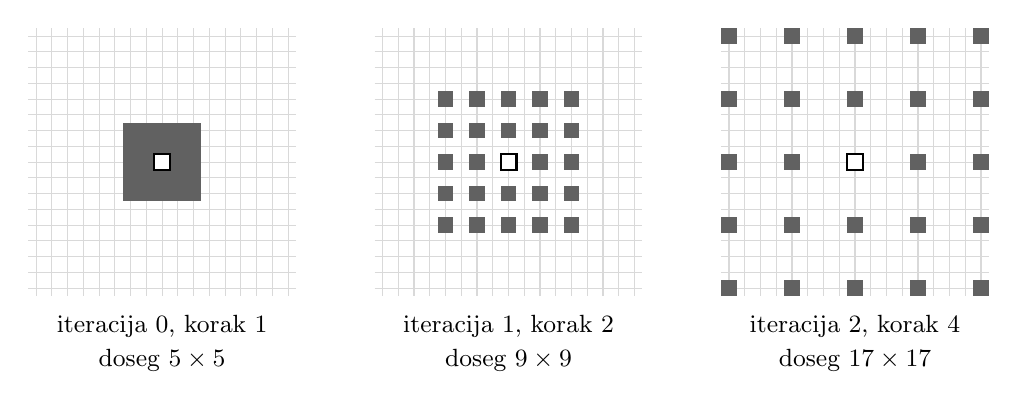
\begin{tikzpicture}[font=\scriptsize, scale=0.2]
  \foreach \it/\stride/\xoff in {0/1/0, 1/2/22, 2/4/44} {
    \begin{scope}[xshift=\xoff cm]
      \draw[black!15] (-8.5,-8.5) grid (8.5,8.5);
      \foreach \dy in {-2,-1,0,1,2} \foreach \dx in {-2,-1,0,1,2} {
        \pgfmathsetmacro{\px}{\dx*\stride}
        \pgfmathsetmacro{\py}{\dy*\stride}
        \fill[black!62] (\px-0.5,\py-0.5) rectangle (\px+0.5,\py+0.5);
      }
      \fill[white] (-0.5,-0.5) rectangle (0.5,0.5);
      \draw[black, thick] (-0.5,-0.5) rectangle (0.5,0.5);
      \node[font=\small] at (0,-10.4) {iteracija \it, korak \stride};
      \node[font=\small] at (0,-12.6) {doseg $\pgfmathparse{int(4*\stride+1)}\pgfmathresult
        \times \pgfmathparse{int(4*\stride+1)}\pgfmathresult$};
    \end{scope}
  }
\end{tikzpicture}
\caption[\`A-trous: rastu\'ci korak i doseg filtra]{Tri iteracije a-trous filtra, sve nad istim
$17\times17$ isecem oko piksela koji se filtrira (beli kvadrat u sredini). Svaka iteracija uzima
istih 25 uzoraka, samo sa dvostruko ve\'cim korakom, pa doseg raste a cena po iteraciji ostaje ista.
Rupe izme\dj u uzoraka su ono \v{c}ime se pla\'ca doseg: kumulativno $29\times29$ za 75 uzoraka
umesto 841.}
\label{fig:atrous}
\end{figure}

Each tap carries three edge-stopping terms (Listing~\ref{lst:atrous}): normal, relative linearized
depth, and the variance-guided luminance term that is the defining idea of SVGF. Because the
luminance weight scales with the square root of the filtered variance, the filter blurs aggressively
where the signal is noisy and preserves detail where it has converged. Variance itself is filtered
with the squared tap weights, and all guide buffers are point-sampled to avoid bleeding across edges.
Disabling the variance term (\texttt{LumaPhi = 0}) reduces the filter to a plain bilateral blur, a
useful baseline in Chapter~\ref{ch:analiza}.


\needspace{12\baselineskip}
\begin{lstlisting}[caption={Edge-stopping te\v{z}ine za \`a-trous filter (SVGF jezgro, HLSL).}, label={lst:atrous}]
float w_n = pow(saturate(dot(N, N_tap)), K_NORMAL);              // normal
float w_z = exp(-abs(z - z_tap) / (K_DEPTH * abs(dzdx) + 1e-4)); // depth
float w_l = exp(-abs(lum - lum_tap) /                            // variance-guided luminance
                (LUMA_PHI * sqrt(varBlur) + 1e-4));
float w   = w_n * w_z * w_l * kernel[dy + 2] * kernel[dx + 2];   // combined tap weight
sum  += w * color_tap;
wSum += w;
\end{lstlisting}

\subsection{Odstupanja od SVGF i cena}

The implementation departs from the paper in a few places, all noted so Chapter~\ref{ch:analiza}'s
quality numbers are read correctly: the denoiser filters raw irradiance and remultiplies albedo after
upsampling rather than demodulating inside the filter as SVGF does; the extra temporal color clamp
above is not in SVGF; GI and AO are filtered at half resolution where SVGF is full-resolution; and
the variance edge-stop is optional. \texttt{GIDenoise.comp} keeps its outer à-trous loop rolled rather
than unrolled, which costs a little scheduling freedom and in exchange holds register pressure down to
70 VGPRs on the RX 7900 XTX and 59 on the RX 9070 XT, with no spilling and full occupancy on both
(Table~\ref{tab:occupancy}). Unrolled it allocates 191 and drops to 8 of 16 wavefronts.

\section{TAA / temporal resolve}
\label{sec:taa}

After the forward pass produces the shaded HDR image, a temporal anti-aliasing resolve \cite{karis2014taa}
(\texttt{TemporalResolvePass}, \texttt{TemporalResolve.frag.hlsl}) accumulates it across frames to
remove aliasing and to converge the residual noise the per-effect denoisers leave behind. The camera
projection is jittered every frame by a Halton(2,3) sequence over a 16-phase cycle. The resolve
reprojects the previous output by the motion vectors (with a closest-depth dilation so thin features
fetch the right velocity), reconstructs the history with a Catmull-Rom filter to reduce reprojection
blur, and clips it against the current $3\times3$ neighborhood in YCoCg space using a Karis
rounded-box bound, loosened for static pixels and tightened under motion.

The resolve runs in linear HDR and does accumulation only. This is a deliberate invariant: any
perceptual or display-space operation (sharpening, contrast) is kept out of this pass and applied
after tonemap, since a per-channel curve applied before tonemap turns an accumulation overshoot into
a hue shift. Sharpening therefore lives in a separate post-tonemap pass, not here.

Motion vectors are the shared prerequisite of three consumers: the SVGF temporal pass, the TAA
resolve, and the screen-space effects that gather last frame's colour. The velocity pass
(Figure~\ref{fig:motion}) renders the scene a second time and writes per pixel the screen-space
displacement of a surface point between the previous and current view-projection matrices.

The failure mode this exposes is disocclusion. A pixel revealed from behind an occluder this frame
has no previous position to point at, so its history is meaningless and reusing it would smear the
occluder's colour across the newly visible surface. Every temporal stage in the engine therefore
pairs the reprojection with a rejection test on depth and normal, and where that test fires the pixel
falls back to the current frame alone, which is noisier but correct.

\begin{figure}[tbp]
\centering
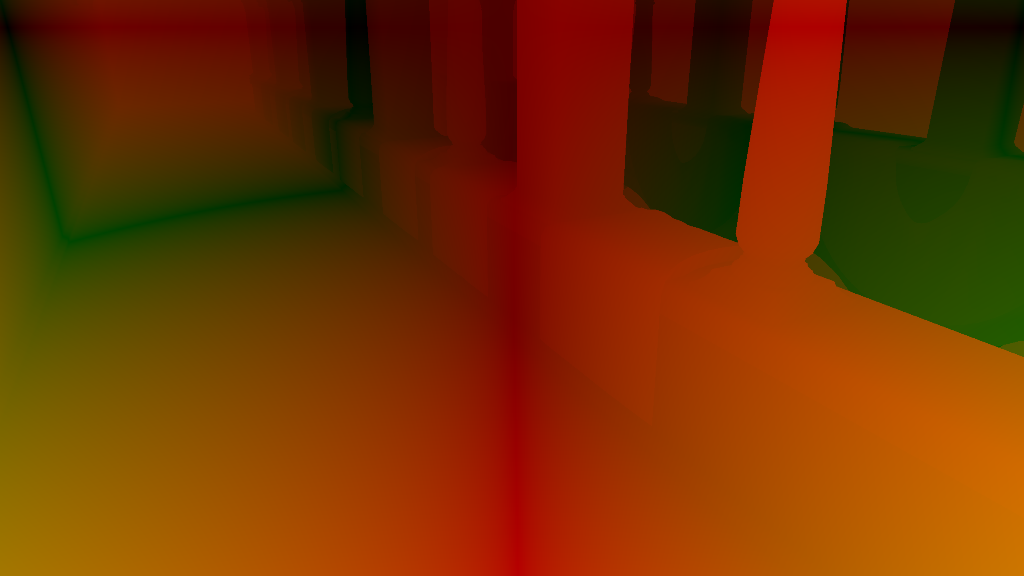
\includegraphics[width=0.8\textwidth]{figures/dbg_motion.png}
\caption{Bafer vektora kretanja (\texttt{render.debugview} 1) tokom determinis\-ti\v{c}ke orbite
kamere. Crveno je vodoravna, zeleno uspravna komponenta pomeraja piksela izme\dj u dva uzastopna
kadra. Prikaz uzima apsolutnu vrednost i mno\v{z}i je sa 40, pa se vidi \emph{koliko} se piksel
pomera i po kojoj osi, ali ne i u kom smeru. Crno je izostanak pomeraja, ali i nebo, koje kroz ovaj
prolaz uop\v{s}te ne upisuje vektore. Prikaz nije kalibrisan: kanali su normirani po \v{s}irini
odnosno visini, pa im osvetljenost nije na istoj skali, a izlaz je jo\v{s} i sRGB kodiran. Kada se
to poni\v{s}ti, prose\v{c}an pomeraj u ovom kadru je oko $0{,}6\%$ dijagonale ekrana po kadru,
najvi\v{s}e $1{,}6\%$, i nijedan uzorak nije zasi\'cen.}
\label{fig:motion}
\end{figure}

\section{Reproducibilnost i alati}
\label{sec:alati}

The measurements in Chapter~\ref{ch:analiza} come from instrumentation built into the engine, which
is what makes them reproducible rather than one-off captures. Every effect is toggled and tuned
through a console-variable registry, so a benchmark configuration is a set of CVar values rather than
a code change, settable from the command line for headless runs, and each render-graph pass is
bracketed by a GPU timestamp scope. Four of the harnesses built on top (Table~\ref{tab:tooling})
compare against a committed baseline and fail the run on a regression, which is what separates a gate
from a report: a number nobody checks drifts.

\begin{table}[tbp]
\caption[Merni alati]{Alati koji proizvode brojeve iz Glave~\ref{ch:analiza}. ,,Kapija`` zna\v{c}i da
alat pore\dj uje sa committovanim baseline-om i obara izvr\v{s}avanje pri regresiji, a alati bez
kapije samo izve\v{s}tavaju. Svi osim \texttt{rga-occupancy} zahtevaju stvarni GPU, pa se izvr\v{s}avaju
lokalno, ne na CI-u.}
\label{tab:tooling}
\centering
\begin{tabular}{lll}
\toprule
Alat & \v{S}ta meri & Kapija \\
\midrule
\texttt{perf-bench}     & GPU ms po prolazu, matrica konfiguracija & da \\
\texttt{quality-bench}  & FLIP/PSNR/SSIM naspram path trace-a, stati\v{c}na kamera & da \\
\texttt{quality-motion} & FLIP, tFLIP, ka\v{s}njenje i JOD du\v{z} rute & da \\
\texttt{rga-occupancy}  & registarski pritisak i zauzetost, offline & da \\
\texttt{quality-tune}   & pretraga CVar-ova prema referenci & ne \\
\texttt{smoke-test}     & pad, zaglavljivanje, Vulkan validacija & pass/fail \\
\texttt{shader-stats}   & registri iz drajvera, oba proizvo\dj a\v{c}a & ne \\
Tracy + watchdog        & vremenska linija po sistemu, zastoji po frejmu & ne \\
\bottomrule
\end{tabular}
\end{table}

\section{Referentni path tracer}
\label{sec:pathtracer}

The reference is a brute-force unidirectional path tracer built into the engine
(\texttt{PathTrace.comp.hlsl}): next-event estimation to the sun, the same metallic-roughness
microfacet BSDF as the forward shading, multi-bounce indirect with Russian-roulette termination, and
progressive accumulation into a persistent HDR buffer while the camera is static. The sun is sampled
as a finite disk through the same \texttt{SampleCone} routine and the same
\texttt{render.shadow.sun\_angle\_deg} half-angle as the real-time soft-shadow path, so any penumbra
difference is attributable to sampling and reconstruction rather than to a different light model (the
sky on a ray miss is added without the sun disk, to avoid double-counting). Because shadows, ambient
occlusion, reflections, and indirect light all emerge from the same multi-bounce transport, one
converged path trace is the ground truth for all of them at once. It converges over many frames and
exists only as the correctness anchor. Both sides of every comparison pass through the same tonemap
chain, so toggling the path tracer is an apples-to-apples A/B rather than a comparison between an HDR
and an LDR image.

\begin{figure}[tbp]
\centering
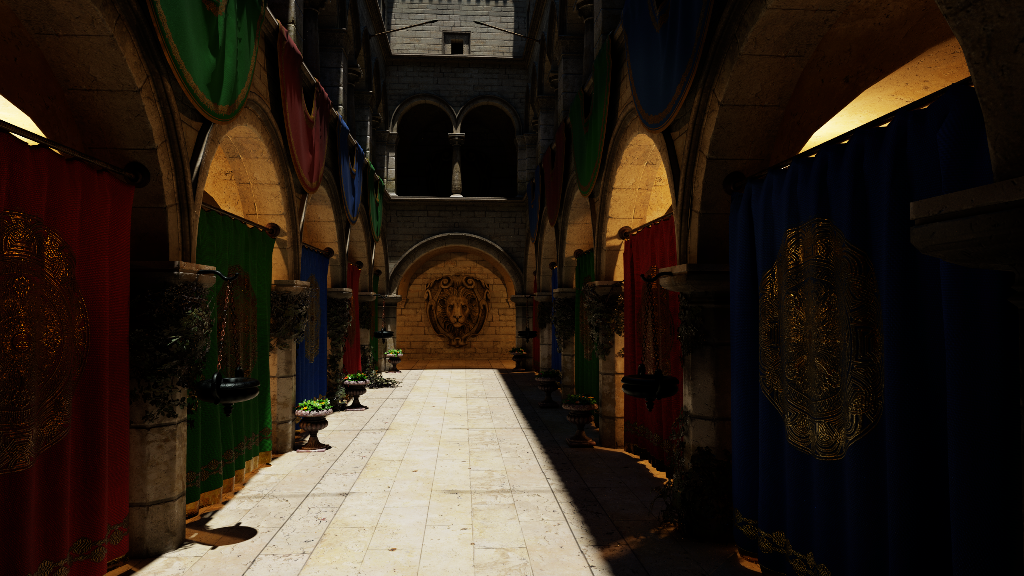
\includegraphics[width=0.85\textwidth]{figures/pt_ref.png}
\caption{Konvergirani referentni kadar iz ugra\dj enog path tracer-a, prema kome se u FLIP/PSNR/SSIM
mere sve real-time tehnike.}
\label{fig:pt-ref}
\end{figure}

\section{Uslovi i pretpostavke}
\label{sec:uslovi}

The implementation makes several deliberate approximations to stay within a real-time budget, each a
simplification of the full problem rather than a factor that distorts the relative measurements in
Chapter~\ref{ch:analiza}.

\begin{itemize}
  \item \textbf{Diffuse, single-bounce GI.} Global illumination computes one diffuse indirect bounce,
    while multi-bounce and glossy indirect are out of scope.
  \item \textbf{Half-resolution GI and AO.} GI and AO are traced at half resolution and bilaterally
    upsampled. Reflections are traced at full resolution.
  \item \textbf{Low sample counts with reconstruction.} Effects use one or two rays per pixel and
    depend on temporal accumulation, and on the spatial SVGF filter for GI and AO, for a usable
    image. The spatial filter is disabled for reflections (Section~\ref{sec:denoise-eval}).
  \item \textbf{Approximate soft shadows.} In the default path ray-traced shadows use one hard or two
    soft rays per light, traced inline and applied directly with no denoiser, so the penumbra is a
    two-sample approximation of an area light cleaned up only by the temporal resolve, not a
    converged soft shadow. The opt-in stochastic path does reconstruct its aggregate visibility
    through the shared denoiser, at the cost of resolving only one light per pixel per frame.
  \item \textbf{Inline ray queries only.} No ray-tracing pipeline, shader binding table, or
    recursion. All hit lighting is a single bounce evaluated in \texttt{ShadeSurfaceHit}.
  \item \textbf{Single-sample local-light NEE, GI only.} A GI secondary hit adds at most one of the
    scene's point and spot lights, importance-picked per hit rather than summed over all of them, so
    it remains a noisy, single-sample estimator of full next-event estimation rather than an exact
    sum. Reflections' hits are not extended with local lights at all (\texttt{render.rt.hit_lights}
    measured no quality gain there for twice the GI-side cost).
  \item \textbf{Full TLAS rebuild per dynamic frame.} The top-level structure is rebuilt, not refit,
    on any frame the scene changes, although a fully static scene skips the rebuild.
\end{itemize}
